%%%%%%%%%%%%%%%%%%%%%%%%%%%%%%%%%%%%%%%%%
% Journal Article
% LaTeX Template
% Version 1.4 (15/5/16)
%
% This template has been downloaded from:
% http://www.LaTeXTemplates.com
%
% Original author:
% Frits Wenneker (http://www.howtotex.com) with extensive modifications by
% Vel (vel@LaTeXTemplates.com)
%
% License:
% CC BY-NC-SA 3.0 (http://creativecommons.org/licenses/by-nc-sa/3.0/)
%
%%%%%%%%%%%%%%%%%%%%%%%%%%%%%%%%%%%%%%%%%

%----------------------------------------------------------------------------------------
%	PACKAGES AND OTHER DOCUMENT CONFIGURATIONS
%----------------------------------------------------------------------------------------

\documentclass[twoside,twocolumn]{article}

\usepackage{blindtext} % Package to generate dummy text throughout this template 

\usepackage{graphicx}

\usepackage[sc]{mathpazo} % Use the Palatino font
\usepackage[T1]{fontenc} % Use 8-bit encoding that has 256 glyphs
\linespread{1.05} % Line spacing - Palatino needs more space between lines
\usepackage{microtype} % Slightly tweak font spacing for aesthetics

\usepackage[english]{babel} % Language hyphenation and typographical rules

\usepackage[hmarginratio=1:1,top=32mm,columnsep=20pt]{geometry} % Document margins
\usepackage[hang, small,labelfont=bf,up,textfont=it,up]{caption} % Custom captions under/above floats in tables or figures
\usepackage{booktabs} % Horizontal rules in tables

\usepackage{lettrine} % The lettrine is the first enlarged letter at the beginning of the text

\usepackage{enumitem} % Customized lists
\setlist[itemize]{noitemsep} % Make itemize lists more compact

\usepackage{abstract} % Allows abstract customization
\renewcommand{\abstractnamefont}{\normalfont\bfseries} % Set the "Abstract" text to bold
\renewcommand{\abstracttextfont}{\normalfont\small\itshape} % Set the abstract itself to small italic text

\usepackage{titlesec} % Allows customization of titles
\renewcommand\thesection{\Roman{section}} % Roman numerals for the sections
\renewcommand\thesubsection{\roman{subsection}} % roman numerals for subsections
\titleformat{\section}[block]{\large\scshape\centering}{\thesection.}{1em}{} % Change the look of the section titles
\titleformat{\subsection}[block]{\large}{\thesubsection.}{1em}{} % Change the look of the section titles

\usepackage{fancyhdr} % Headers and footers
\pagestyle{fancy} % All pages have headers and footers
\fancyhead{} % Blank out the default header
\fancyfoot{} % Blank out the default footer
%\fancyhead[C]{Running title $\bullet$ May 2016 $\bullet$ Vol. XXI, No. 1} % Custom header text
\fancyfoot[RO,LE]{\thepage} % Custom footer text

\usepackage{titling} % Customizing the title section

\usepackage{hyperref} % For hyperlinks in the PDF
\usepackage{amsmath}

%----------------------------------------------------------------------------------------
%	TITLE SECTION
%----------------------------------------------------------------------------------------

\setlength{\droptitle}{-4\baselineskip} % Move the title up

\pretitle{\begin{center}\Huge\bfseries} % Article title formatting
\posttitle{\end{center}} % Article title closing formatting
\title{Implementation of A Fully connected Neural Network Using Numpy} % Article title
\author{%
\textsc{Haocong Wang} \\[1ex] % Your name
%\normalsize University of California \\ % Your institution
\normalsize {mw814@scarletmail.rutgers.edu} % Your email address
%\and % Uncomment if 2 authors are required, duplicate these 4 lines if more
%\textsc{Jane Smith}\thanks{Corresponding author} \\[1ex] % Second author's name
%\normalsize University of Utah \\ % Second author's institution
%\normalsize \href{mailto:jane@smith.com}{jane@smith.com} % Second author's email address
}
\date{\today} % Leave empty to omit a date
\renewcommand{\maketitlehookd}{%
\begin{abstract}
\noindent In this project, we design and implement a fully connected neural network using numpy. The network we finished is a four-layer network. All the codes are finished on PyCharm with Python 3.7.8. We choose the MINST dataset to train and test our model. Finally, the result shows that our model can reach the accuracy above 90\%, which fulfills the requirement. % Dummy abstract text - replace \blindtext with your abstract text
\end{abstract}
}

%----------------------------------------------------------------------------------------

\begin{document}

% Print the title
\maketitle

%----------------------------------------------------------------------------------------
%	ARTICLE CONTENTS
%----------------------------------------------------------------------------------------

\section{Introduction}~\label{sec:intro}

%\lettrine[nindent=0em,lines=3]{B} 
A neural network is a network or circuit of neurons, or in a modern sense, an artificial neural network, composed of artificial neurons or nodes, as shown in figure~\ref{fig:nn}. Thus a neural network is either a biological neural network, made up of real biological neurons, or an artificial neural network, for solving artificial intelligence (AI) problems \cite{nn}. The connections of the biological neuron are modeled as weights. A positive weight reflects an excitatory connection, while negative values mean inhibitory connections. All inputs are modified by a weight and summed. This activity is referred to as a linear combination. Finally, an activation function controls the amplitude of the output.

Fully connected neural networks (FCNNs) are a type of artificial neural network where the architecture is such that all the nodes, or neurons, in one layer are connected to the neurons in the next layer \cite{fcnn}, as shown in figure~\ref{fig:fcnn}. 

\begin{figure}
	\centering
	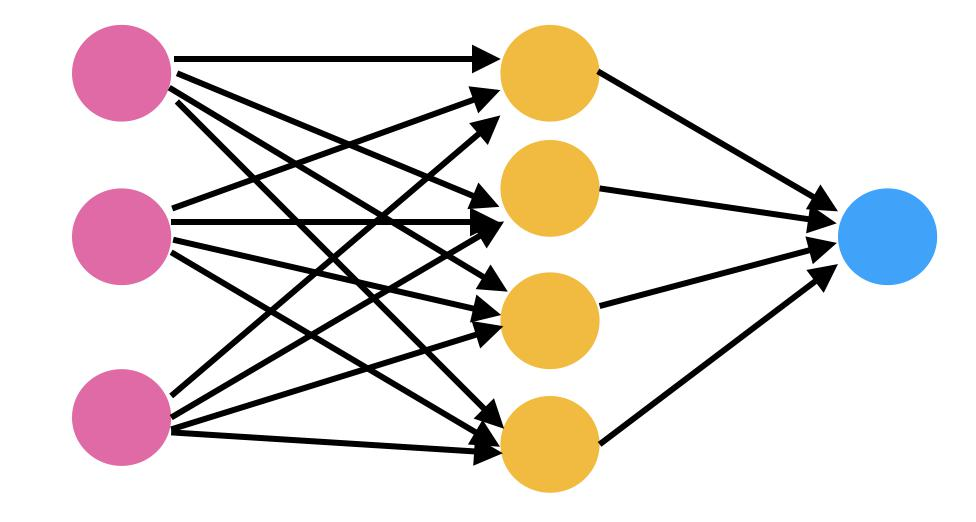
\includegraphics[width=1.0\columnwidth, clip=true]{fig/nn.jpg}
	\vspace{-4mm}
	\caption{A simple neural network.}
	\label{fig:nn}
	\vspace{-5mm}
\end{figure}

\begin{figure}
	\centering
	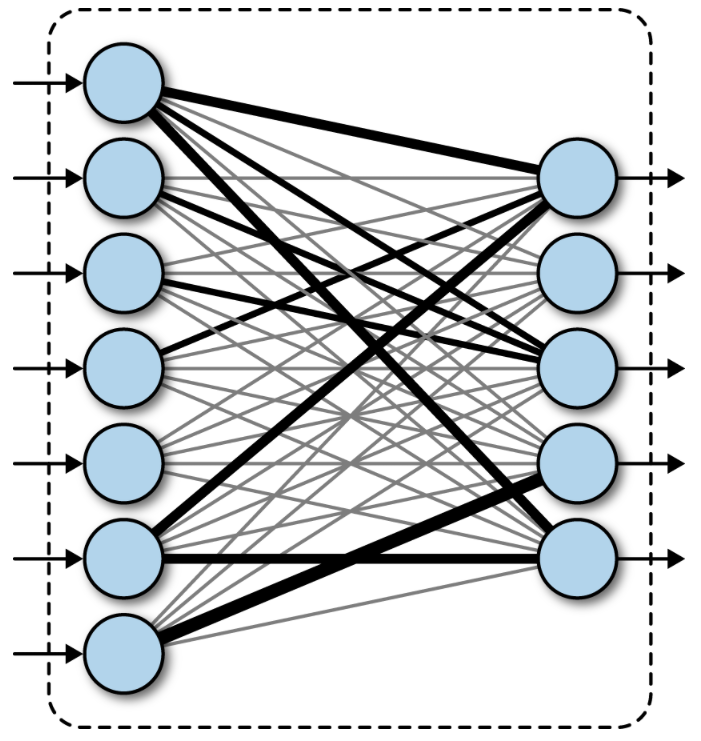
\includegraphics[width=1.0\columnwidth, clip=true]{fig/fcnn.png}
	\vspace{-4mm}
	\caption{A fully connected neural network.}
	\label{fig:fcnn}
	\vspace{-5mm}
\end{figure}

FCNNs have great potential in image recognition. In image recognition, digits recognition is one of the basic applications. So in this project, we design and implement a $784 \times 200 \times 10 \times 1$ network using the MINST dataset, which contains a large number of handwritten digits from 0-9 that are commonly used for training various image processing systems. The result shows that the accuracy can reach above 90\% after the training process is completed.

%------------------------------------------------

\section{Related Work}~\label{sec:related}

\subsection{Gradient Descent}

Gradient descent is a first-order iterative optimization algorithm for finding a local minimum of a differentiable function \cite{gradient}. The idea is to take repeated steps in the opposite direction of the gradient (or approximate gradient) of the function at the current point, because this is the direction of steepest descent, as shown in figure~\ref{fig:grad}.

\subsection{Backpropagation}

In machine learning, backpropagation (BP) is a widely used algorithm for training feed-forward neural networks \cite{lecun1988theoretical}. In fitting a neural network, backpropagation computes the gradient of the loss function with respect to the weights of the network for a single input–output example, and does so efficiently, unlike a naive direct computation of the gradient with respect to each weight individually.

\begin{figure}[h]
	\centering
	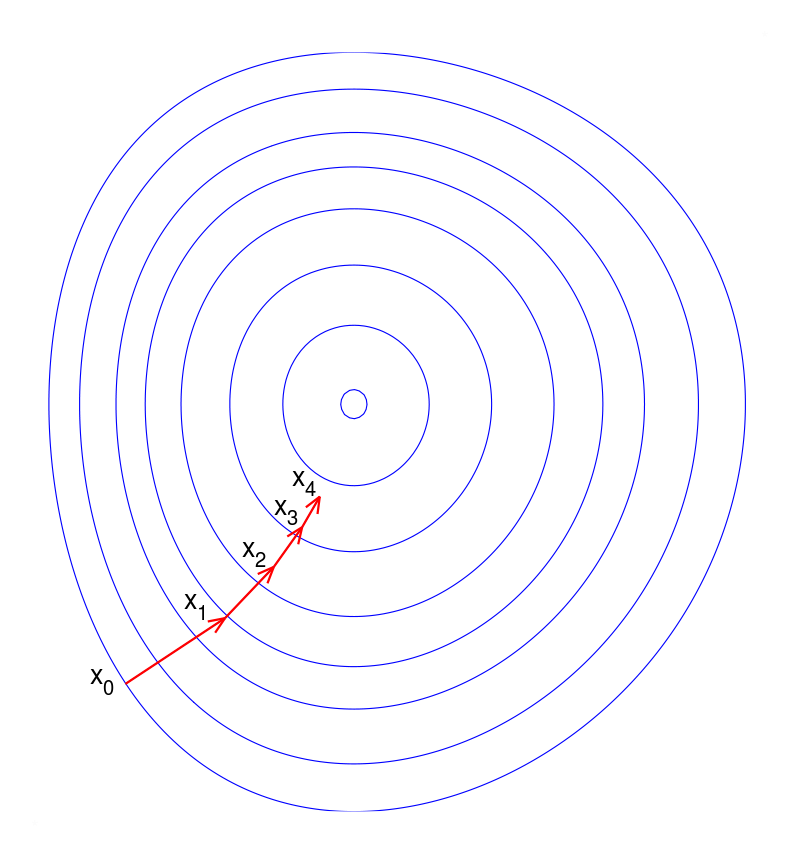
\includegraphics[width=1.0\columnwidth, clip=true]{fig/Gradient_descent.png}
	\vspace{-4mm}
	\caption{Gradient Descent.}
	\label{fig:grad}
	\vspace{-5mm}
\end{figure}

%------------------------------------------------

\section{Description of Dataset, Method and Model}~\label{sec:des}

%\begin{itemize}
%\item Donec dolor arcu, rutrum id molestie in, viverra sed diam
%\item Curabitur feugiat
%\item turpis sed auctor facilisis
%\item arcu eros accumsan lorem, at posuere mi diam sit amet tortor
%\item Fusce fermentum, mi sit amet euismod rutrum
%\item sem lorem molestie diam, iaculis aliquet sapien tortor non nisi
%\item Pellentesque bibendum pretium aliquet
%\end{itemize}
%\blindtext % Dummy text

%Text requiring further explanation\footnote{Example footnote}.

In this section, we will discuss the details of the dataset, method and model used in our project.

\subsection{Dataset}

The dataset we are using is MNIST \cite{lecun1998mnist}. This is a large dataset of handwritten digits from 0-9 that are commonly used for training various image processing systems. All these numbers are from 250 different people, 50\% of who are middle school students, and another 50\% of who are faculty of the Census Bureau. The dataset itself is divided into a training set that has 60000 samples and a testing set with 10000 samples. Each image in this dataset has $28 \times 28$ pixels. So in the training process, we flat each image into a 784 dimension vector. The examples are shown in figure~\ref{fig:mnist}.

\begin{figure}[]
	\centering
	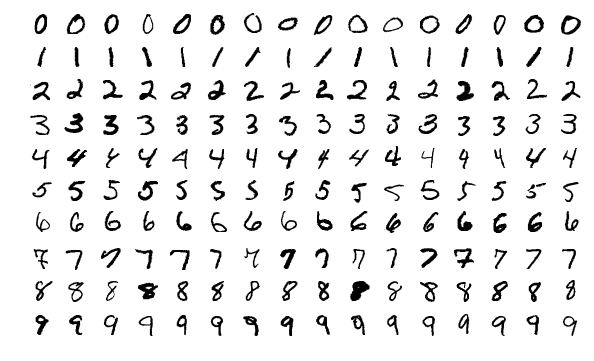
\includegraphics[width=1.0\columnwidth, clip=true]{fig/mnist.png}
	\vspace{-4mm}
	\caption{An image from the MNIST dataset.}
	\label{fig:mnist}
	\vspace{-5mm}
\end{figure}

\subsection{Method}

In this section, we provide detailed introduction for all the mathematical methods used in our model, which includes ReLu Function, Softmax Function and Loss Function.

\begin{figure*}[ht]
	\centering
	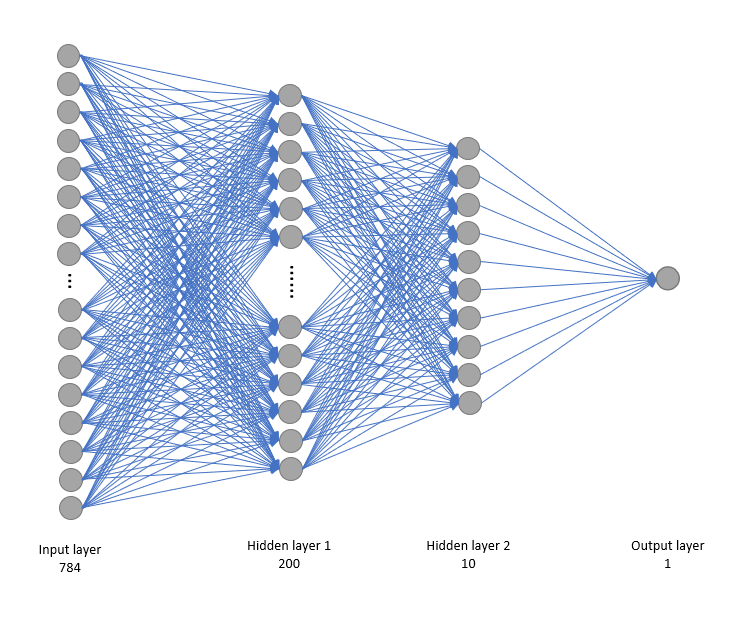
\includegraphics[scale=0.5, clip=true]{fig/network.png}
	\vspace{-2mm}
	\caption{The review of our network.}
	\label{fig:model}
	\vspace{-5mm}
\end{figure*}

\subsubsection{ReLu Function}

For the ReLU Function, we decide use the Ramp function, which is a widely used rectifier
in the machine learning field \cite{relu}. As its name showed, the graph of ramp function looks like a ramp. And can be described mathematically as follow:

\begin{equation}
	R(x):=max(0,x)
\end{equation}

The backward computation of this function can be seen as:

\begin{equation}
	\frac{dr_i}{dx_i}=\left\{
	\begin{aligned}
		&0, x_i\leq 0\\
		&1, x_i> 0
	\end{aligned}
	\right.
\end{equation}

\subsubsection{Softmax Function}

The Softmax function \cite{softmax} takes input as a vector of k real numbers and normalizes it into a probability distribution consisting of K probabilities proportional to the exponential of the input numbers. And it can be mathematically defined as follow:

\begin{equation}
	\sigma(z)_i = \frac{e^{z_i}}{\sum_{j=i}^K e^{z_i}}
\end{equation}

\subsubsection{Loss Function}

We decide to use cross-entropy as our loss function. The cross-entropy \cite{cross} between two probability distributions p and q over the same underlying set of events measures the average number of bits needed to identify an event drawn from the set if a coding scheme used for the set is optimized for an estimated probability distribution q, rather than the true distribution p.

\begin{equation*}
	H(p,q) = -\sum_{i=1}^n p(x_i)log(q(x_i))
\end{equation*}

\subsection{Model}

As mentioned in Section~\ref{sec:intro}, we build a four-layer fully connected neural network, as shown in figure~\ref{fig:model}. Considering the image data that will be taken as input, the first layer has 784 neurons and will output 200 neurons. The two hidden layers have 200 and 10 dimensions, respectively.

%------------------------------------------------

\begin{figure*}[t]
	\centering
	\begin{minipage}[t]{0.3\textwidth}
		\centering
		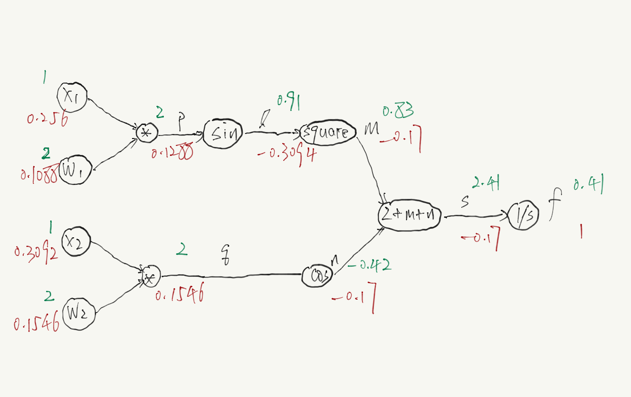
\includegraphics[scale=0.7, clip=true]{fig/1.png}
	\end{minipage}
	\begin{minipage}[t]{0.3\textwidth}
		\centering
		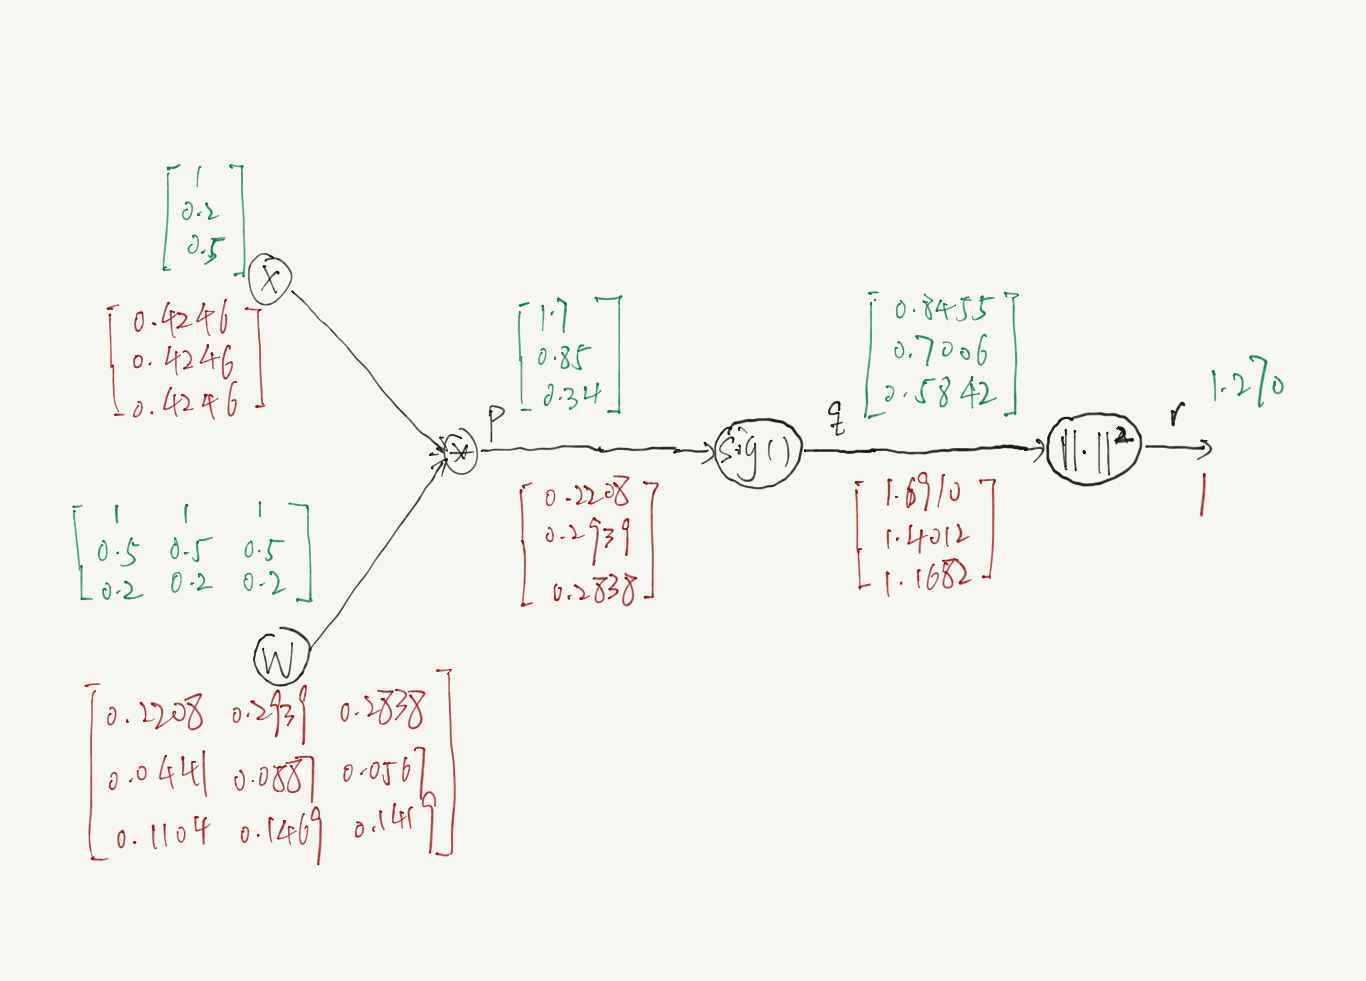
\includegraphics[scale=0.7, clip=true]{fig/2.png}
	\end{minipage}
	\begin{minipage}[t]{0.3\textwidth}
		\centering
		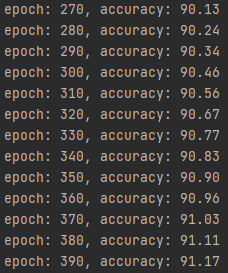
\includegraphics[scale=0.7, clip=true]{fig/3.png}
	\end{minipage}
	\vspace{-2mm}
	\caption{Epochs of training.}
	\label{fig:epoch}
	\vspace{-2mm}
\end{figure*}

\begin{figure*}[ht]
	\centering
	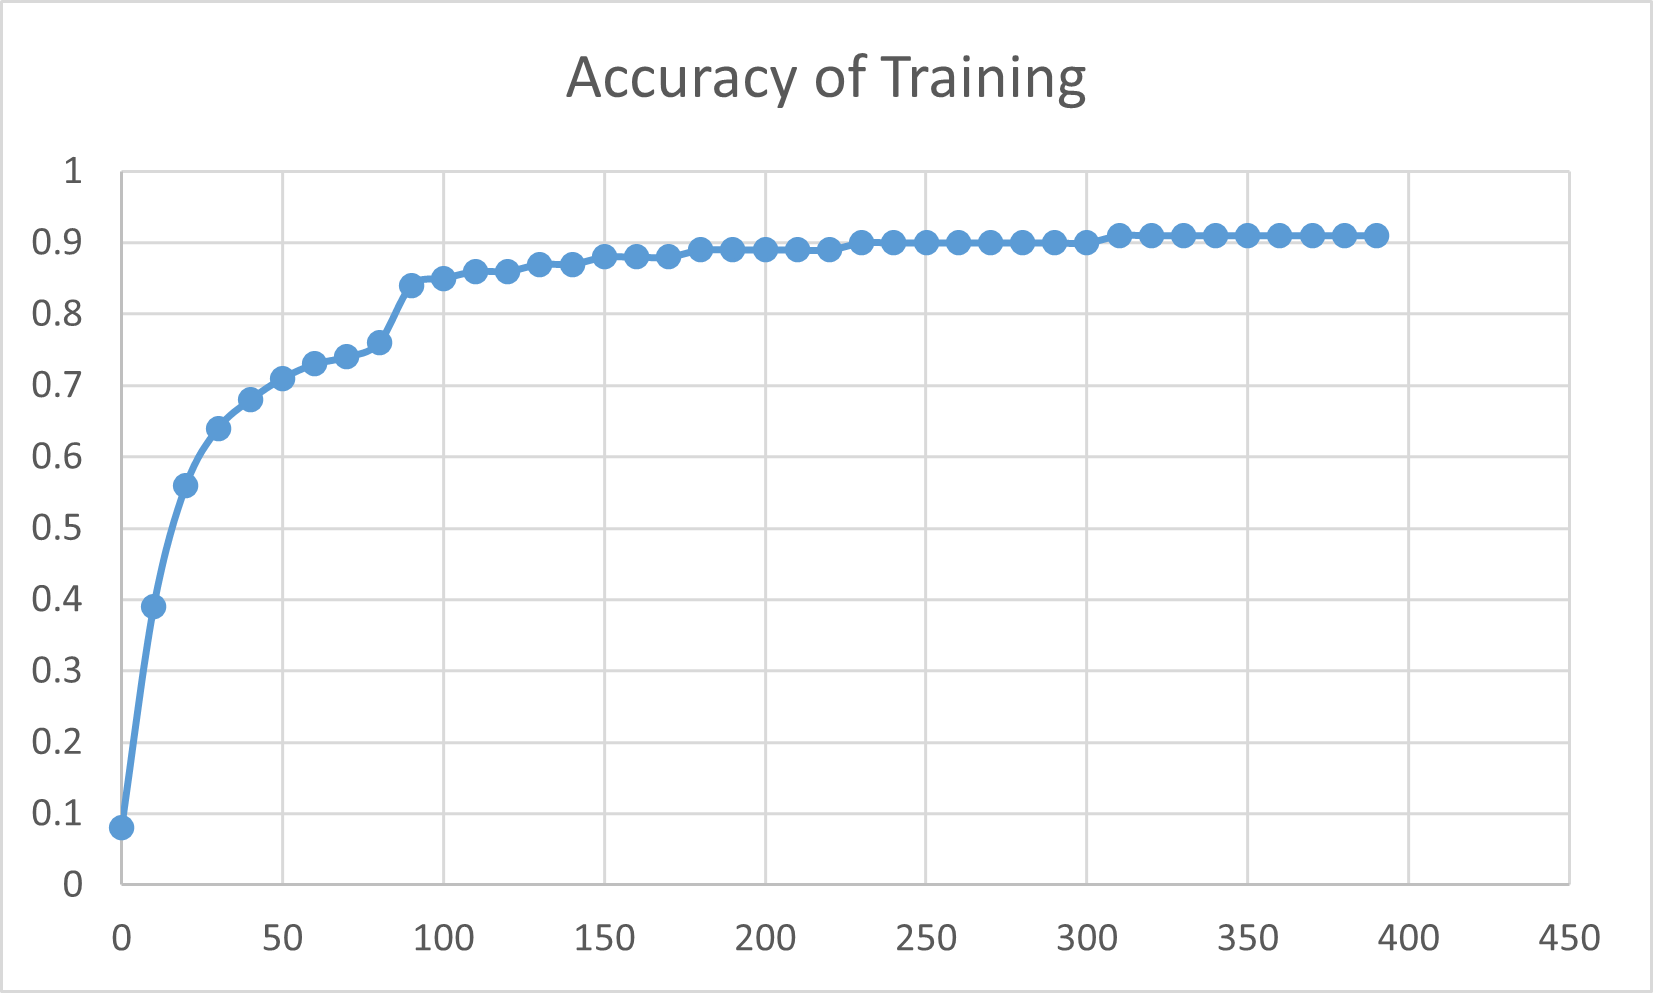
\includegraphics[scale=0.9, clip=true]{fig/Result.png}
	\vspace{-2mm}
	\caption{The trend of accuracy.}
	\label{fig:trend}
	\vspace{-5mm}
\end{figure*}

\section{Experimental Procedure and Results}

We use numpy to build the model on PyCharm. We first set the epochs of training to be 1000, but then we found that after the accuracy reaches 80\%, the speed of increasing accuracy starts to slow down. Therefore, we finally choose 400 as the epochs of training, as shown in figure~\ref{fig:epoch}.

After 400 times of training, we test the trained model on the testing dataset extracted from the MNIST dataset. The accuracy is finally stabilized at around 90\%, as shown in figure~\ref{fig:accu}. We also show the trend of the accuracy during training in figure~\ref{fig:trend}. As can be seen from the figure, the accuracy reach above 90\% at around 200 epochs. There is another point in our project. Since we initiate the weights and bias randomly, the process might be much slower if we are unfortunate to initiate a series of bad weights.

\begin{figure}[]
	\centering
	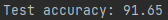
\includegraphics[width=0.75\columnwidth, clip=true]{fig/4.png}
	\vspace{-2mm}
	\caption{The final accuracy.}
	\label{fig:accu}
	\vspace{-5mm}
\end{figure}

%\begin{equation}
%\label{eq:emc}
%e = mc^2
%\end{equation}

%------------------------------------------------

\section{Conclusion}

In this project, we design and implement a four-layer fully connected neural network with numpy. We choose MNIST as our dataset and finish 400 epochs of training. The results show that the accuracy can reach above 90\%. % Dummy text

%----------------------------------------------------------------------------------------
%	REFERENCE LIST
%----------------------------------------------------------------------------------------

%\begin{thebibliography}{99} % Bibliography - this is intentionally simple in this template

\bibliographystyle{abbrv}
\bibliography{bib}

%\bibitem[Figueredo and Wolf, 2009]{Figueredo:2009dg}
%Figueredo, A.~J. and Wolf, P. S.~A. (2009).
%\newblock Assortative pairing and life history strategy - a cross-cultural
%  study.
%\newblock {\em Human Nature}, 20:317--330.
 
%\end{thebibliography}

%----------------------------------------------------------------------------------------

\end{document}
